% En images.tex
\DeclareRobustCommand{\squashedplot}{
\begin{figure}[H]
    \centering
    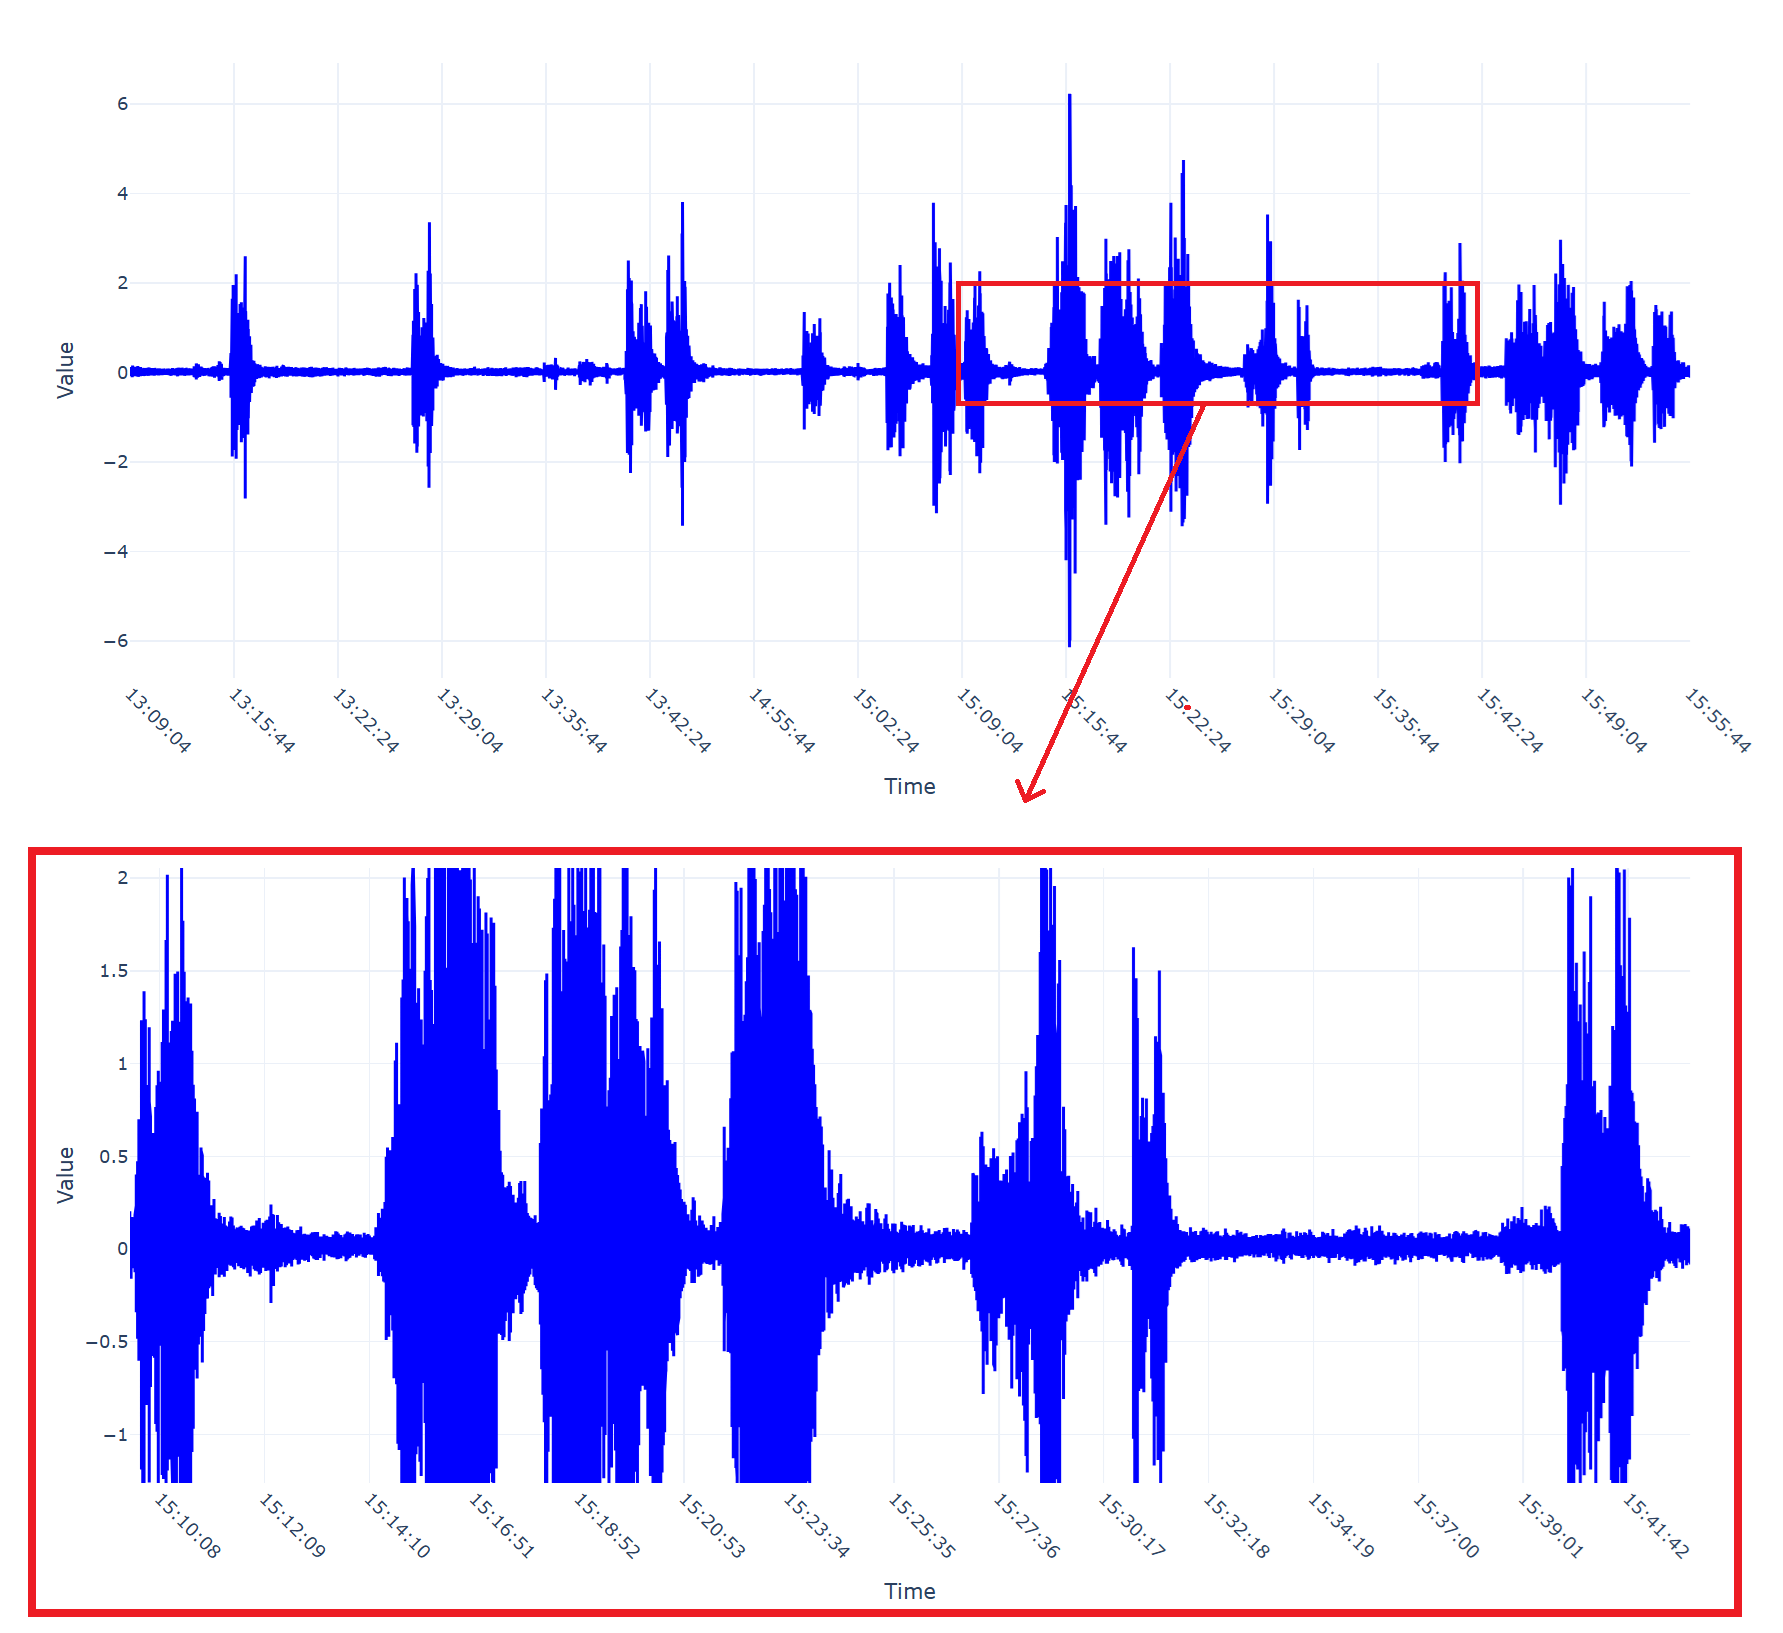
\includegraphics[width=0.9\linewidth]{introduction/images/squashed_plot.png}
    \caption[Serie comprimida del sensor]{Serie de tiempo con aproximadamente 350,000 puntos con valores del sensor de un puente. Al ser demasiados puntos por segundo, es difícil identificar el comportamiento del sensor en cada segundo.}
    \label{squashed_plot}
\end{figure}
}

\DeclareRobustCommand{\downsample}{
\begin{figure}[H]
    \centering
    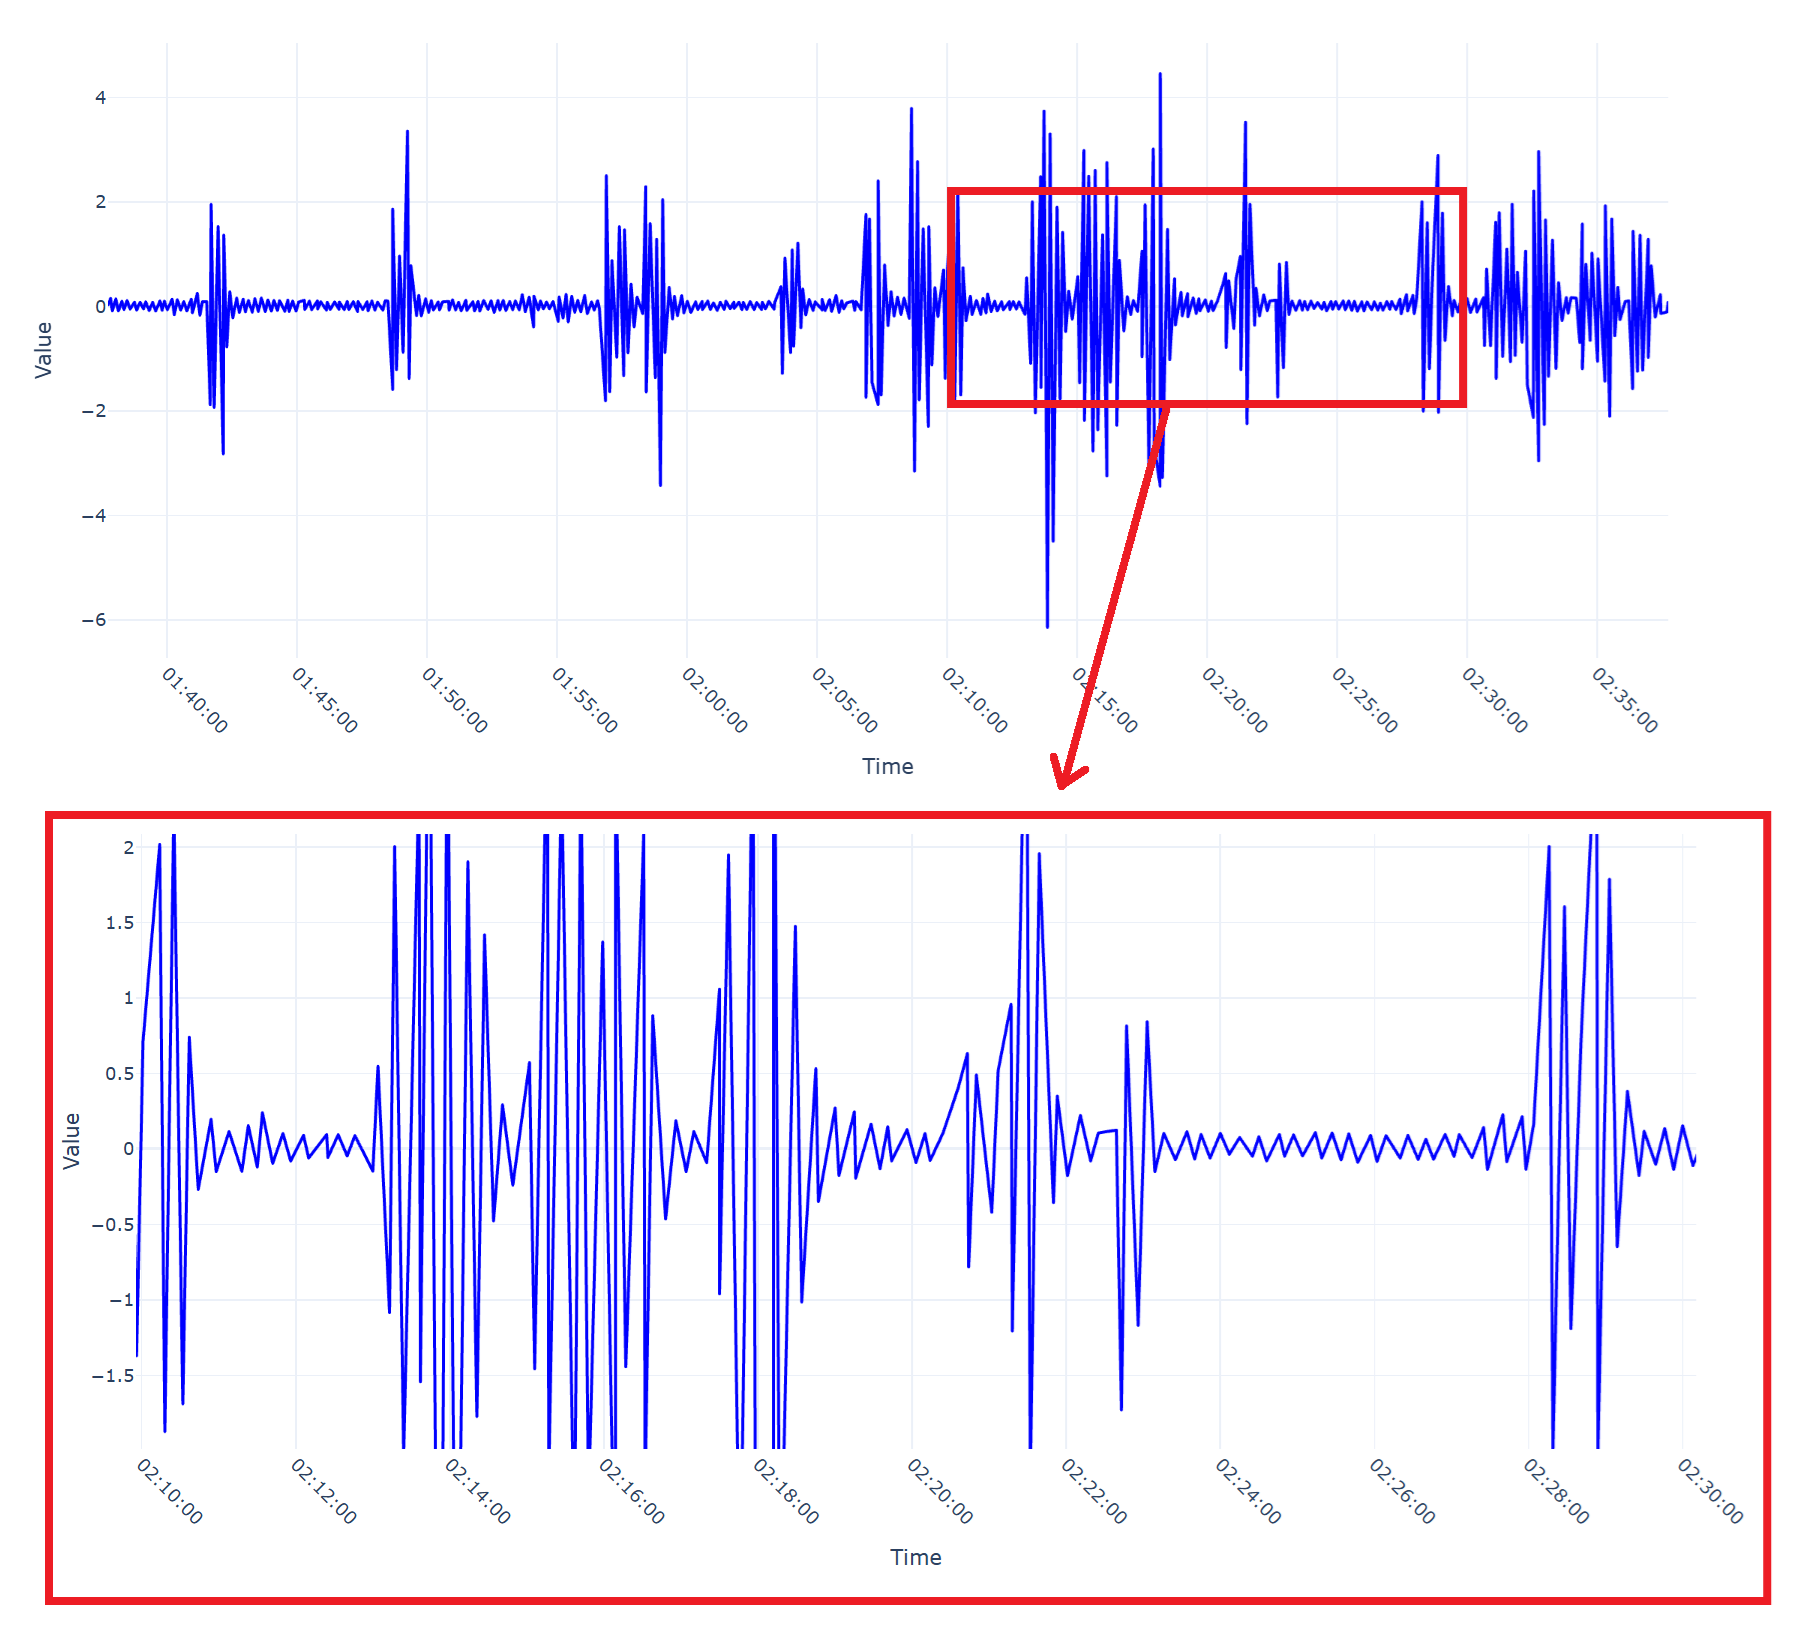
\includegraphics[width=0.9\linewidth]{introduction/images/downsample.png}
    \caption[Downsample de serie de tiempo]{Downsample de serie de tiempo con aproximadamente 350,000 puntos con valores del sensor de un puente.}
    \label{downsample}
\end{figure}
}

\DeclareRobustCommand{\plotlyresampler}{
\begin{figure}
    \centering
    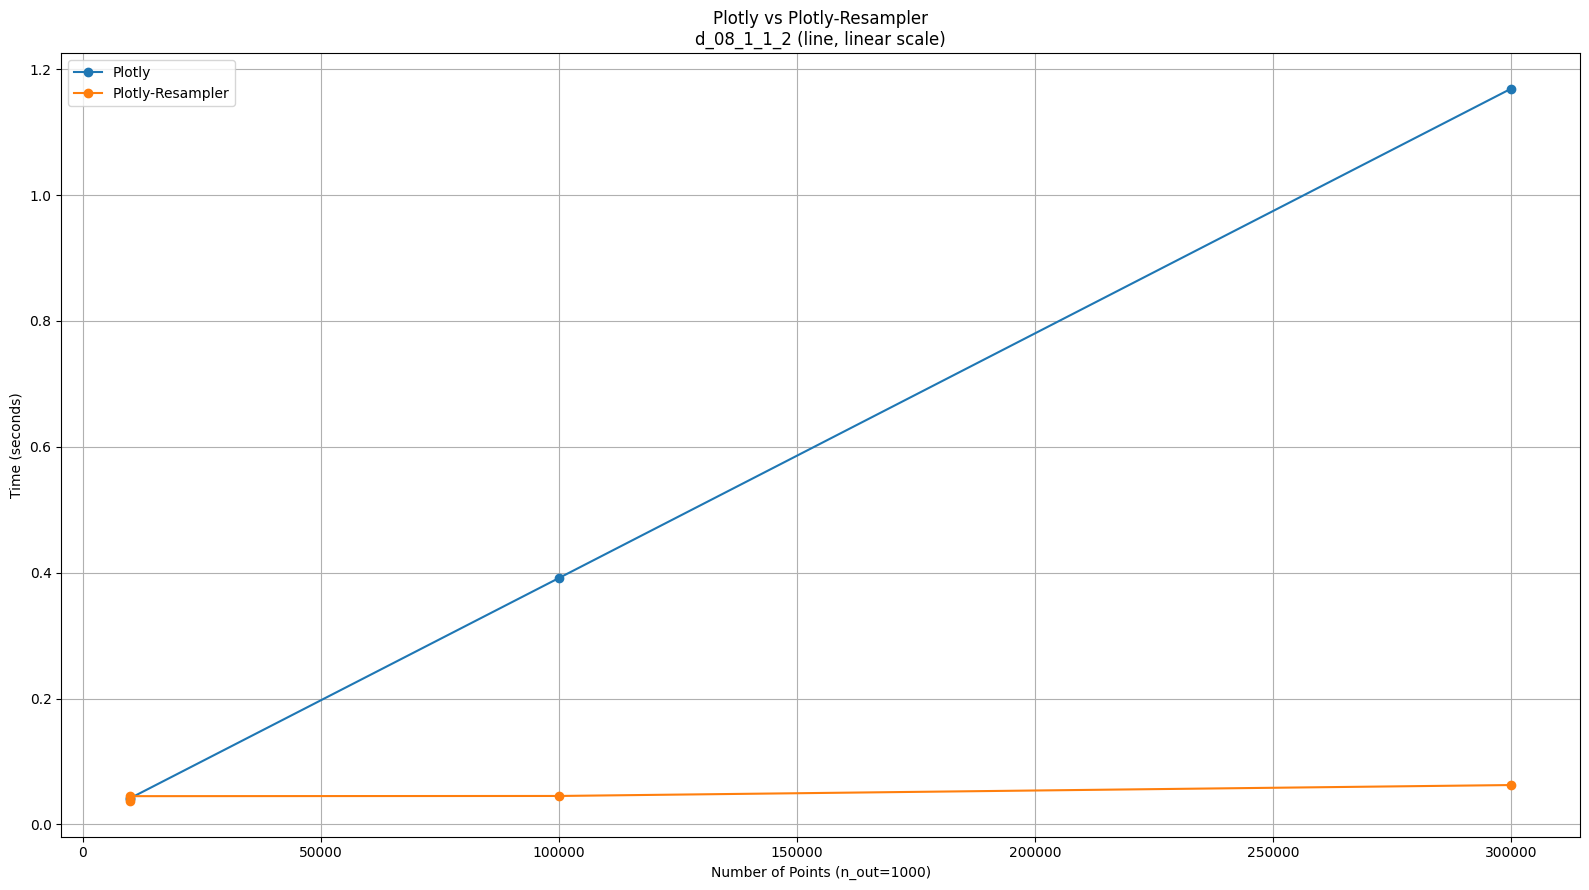
\includegraphics[width=0.9\linewidth]{introduction/images/plotly_resampler.png}
    \caption[Tiempo de Renderizado Plotly vs Plotly-Resampler]{Comparación de tiempo entre las librerias \textit{plotly} y \textit{plotly-resampler} al crear gráficos con $n$ cantidad de puntos.}
    \label{plotly_vs_resampler}
\end{figure}
}
% \DeclareRobustCommand{}{

% }
% \DeclareRobustCommand{}{

% }
% \DeclareRobustCommand{}{

% }
% \DeclareRobustCommand{}{

% }
% \DeclareRobustCommand{}{

% }
% \DeclareRobustCommand{}{

% }
% \DeclareRobustCommand{}{

% }
% \DeclareRobustCommand{}{

% }
% \DeclareRobustCommand{}{

% }
